\documentclass[tikz,border=4pt]{standalone}
\usepackage{xcolor}
\definecolor{journalink}{HTML}{1F1C18}
\begin{document}
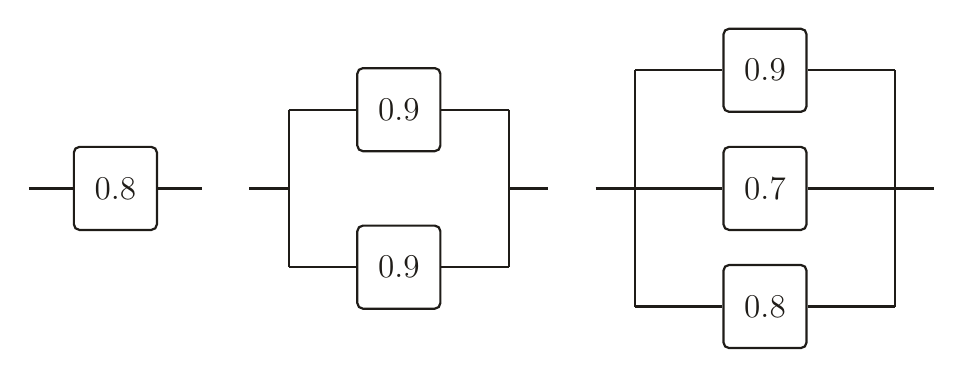
\begin{tikzpicture}[-,auto,node distance=1cm,
  point/.style={coordinate},
  block/.style={draw=journalink, line width=0.8pt, rounded corners=2pt, rectangle, minimum height=3em, minimum width=3em, text=journalink, font=\large},
  every path/.style={draw=journalink, line width=0.8pt}]
\begin{scope}[shift={(0,0)}]
\node[point] (a0) at (-2.2,0)  {};
\node[block] (a1) at (-1.1,0)  {0.8};
\node[point] (a2) at (0,0)  {};
\draw   (a0) -- (a1);
\draw   (a1) -- (a2);
\end{scope}
\begin{scope}[shift={(0.6,0)}]
\node[point] (b0) at (0,0)  {};
\node[point] (b1) at (0.5,0)  {};
\node[point] (b2) at (0.5,1)  {};
\node[block] (b3) at (1.9,1)  {0.9};
\node[point] (b4) at (3.3,1)  {};
\node[point] (b5) at (0.5,-1)  {};
\node[block] (b6) at (1.9,-1)  {0.9};
\node[point] (b7) at (3.3,-1)  {};
\node[point] (b8) at (3.3,0)  {};
\node[point] (b9) at (3.8,0)  {};
\draw   (b0) -- (b1);
\draw   (b1) -- (b2);
\draw   (b1) -- (b5);
\draw   (b2) -- (b3);
\draw   (b3) -- (b4);
\draw   (b5) -- (b6);
\draw   (b6) -- (b7);
\draw   (b7) -- (b8);
\draw   (b4) -- (b8);
\draw   (b8) -- (b9);
\end{scope}
\begin{scope}[shift={(5.5,0)}]
\node[point] (c8) at (-0.5,0)  {};
\node[point] (c9) at (0,0)  {};
\node[point] (c10) at (0,1.5)  {};
\node[block] (c11) at (1.65,1.5)  {0.9};
\node[point] (c12) at (3.3,1.5)  {};
\node[point] (c13) at (0,-1.5)  {};
\node[block] (c14) at (1.65,-1.5)  {0.8};
\node[point] (c15) at (3.3,-1.5)  {};
\node[block] (c16) at (1.65,0)  {0.7};
\node[point] (c17) at (3.3,0)  {};
\node[point] (c18) at (3.8,0)  {};
\draw   (c8) -- (c9);
\draw   (c9) -- (c10);
\draw   (c10) -- (c11);
\draw   (c11) -- (c12);
\draw   (c9) -- (c13);
\draw   (c13) -- (c14);
\draw   (c14) -- (c15);
\draw   (c9) -- (c16);
\draw   (c16) -- (c17);
\draw   (c12) -- (c17);
\draw   (c15) -- (c17);
\draw   (c17) -- (c18);
\end{scope}
\end{tikzpicture}
\end{document}
